% Dokumentenart. Ersetze 12pt, falls die Schriftgröße anzupassen ist.
\documentclass[12pt]{scrartcl}

% Einbinden der Pakete, des Headers und der Formatierung.
% LaTeX Template für Abgaben an der Universität Stuttgart
% Autor: Sandro Speth
% Bei Fragen: Sandro.Speth@studi.informatik.uni-stuttgart.de
%-----------------------------------------------------------
% Modul fuer verwendete Pakete.
% Neue Pakete einfach einfuegen mit dem \usepackage Befehl:
% \usepackage[options]{packagename}
\usepackage[utf8]{inputenc}
\usepackage[T1]{fontenc}
\usepackage[ngerman]{babel}
\usepackage{lmodern}
\usepackage{graphicx}
\usepackage{float}
\usepackage[pdftex,hyperref,dvipsnames]{xcolor}
\usepackage{listings}
\usepackage[a4paper,lmargin={2cm},rmargin={2cm},tmargin={3.5cm},bmargin = {2.5cm},headheight = {4cm}]{geometry}
\usepackage{amsmath,amssymb,amstext,amsthm}
\usepackage[lined,algonl,boxed]{algorithm2e}
\usepackage{algorithmic}
\usepackage{multirow}
% alternative zu algorithm2e:
%\usepackage[]{algorithm} %counter mit chapter
%\usepackage{algpseudocode}
\usepackage{tikz}
\usepackage{hyperref}
\usepackage{url}
\usepackage[inline]{enumitem} % Ermöglicht ändern der enum Item Zahlen
\usepackage[headsepline]{scrlayer-scrpage} 
\usepackage{csquotes}
\pagestyle{scrheadings} 
\usetikzlibrary{automata,positioning,shapes.geometric,trees}

% LaTeX Template für Abgaben an der Universität Stuttgart
% Autor: Sandro Speth
% Bei Fragen: Sandro.Speth@studi.informatik.uni-stuttgart.de
%-----------------------------------------------------------
% Modul beinhaltet Befehl fuer Aufgabennummerierung,
% sowie die Header Informationen.

% Überschreibt enumerate Befehl, sodass 1. Ebene Items mit
\renewcommand{\theenumi}{(\alph{enumi})}
\renewcommand{\theenumii}{(\roman{enumii})}
% (a), (b), etc. nummeriert werden.
\renewcommand{\labelenumi}{\text{\theenumi}}
\renewcommand{\labelenumii}{\text{\theenumii}}

% Counter für das Blatt und die Aufgabennummer.
% Ersetze die Nummer des Übungsblattes und die Nummer der Aufgabe
% den Anforderungen entsprechend.
% Gesetz werden die counter in der hauptdatei, damit siese hier nicht jedes mal verändert werden muss
% Beachte:
% \setcounter{countername}{number}: Legt den Wert des Counters fest
% \stepcounter{countername}: Erhöht den Wert des Counters um 1.
\newcounter{sheetnr}
\newcounter{exnum}

% Befehl für die Aufgabentitel
\newcommand{\exercise}[1]{\section*{Exercise \theexnum\stepcounter{exnum}: #1}} % Befehl für Aufgabentitel

% Formatierung der Kopfzeile
% \ohead: Setzt rechten Teil der Kopfzeile mit
% Namen und Matrikelnummern aller Bearbeiter
\ohead{Hui Zeng}
% \chead{} kann mittleren Kopfzeilen Teil sezten
% \ihead: Setzt linken Teil der Kopfzeile mit
% Modulnamen, Semester und Übungsblattnummer
\ihead{Cloud Computing\\
Summer semester 2021\\
Lecture Notes Summary}

\definecolor{comments}{rgb}{0.41,0.54,0.21}
\definecolor{code}{rgb}{0,0,0}
\definecolor{keyword}{rgb}{0.77,0.48,0.57}
\definecolor{number}{rgb}{0.153,0.5,0}
\definecolor{codeBack}{rgb}{0.85,0.85,0.85}
\definecolor{string}{rgb}{0.81,0.57,0.47}

\lstdefinestyle{stdCode}{
	backgroundcolor=\color{codeBack},   
	commentstyle=\color{comments},
	literate=*{0}{{\textcolor{number}{0}}}{1}%
         {1}{{\textcolor{number}{1}}}{1}%
         {2}{{\textcolor{number}{2}}}{1}%
         {3}{{\textcolor{number}{3}}}{1}%
         {4}{{\textcolor{number}{4}}}{1}%
         {5}{{\textcolor{number}{5}}}{1}%
         {6}{{\textcolor{number}{6}}}{1}%
         {7}{{\textcolor{number}{7}}}{1}%
         {8}{{\textcolor{number}{8}}}{1}%
         {9}{{\textcolor{number}{9}}}{1}%
         {.0}{{\textcolor{number}{.0}}}{1}% Following is to ensure that only periods
         {.1}{{\textcolor{number}{.1}}}{1}% followed by a digit are changed.
         {.2}{{\textcolor{number}{.2}}}{1}%
         {.3}{{\textcolor{number}{.3}}}{1}%
         {.4}{{\textcolor{number}{.4}}}{1}%
         {.5}{{\textcolor{number}{.5}}}{1}%
         {.6}{{\textcolor{number}{.6}}}{1}%
         {.7}{{\textcolor{number}{.7}}}{1}%
         {.8}{{\textcolor{number}{.8}}}{1}%
         {.9}{{\textcolor{number}{.9}}}{1}%
         {\ }{{ }}{1}% handle the space
         ,%
	keywordstyle=\color{keyword},
	numberstyle=\tiny\color{number},
	stringstyle=\color{string},
	basicstyle=\ttfamily\scriptsize,
	breakatwhitespace=false,         
	breaklines=true,                 
	captionpos=b,                    
	keepspaces=true,                 
	numbers=left,                    
	numbersep=5pt,                  
	showspaces=false,                
	showstringspaces=false,
	showtabs=false,                  
	tabsize=2
}

\lstset{
	style=stdCode, language=Java,
  	literate={ö}{{\"o}}1
           {ä}{{\"a}}1
           {ü}{{\"u}}1
}

\tikzset{triangle/.style = {regular polygon, regular polygon sides=3 },
node rotated/.style = {rotate=180},
border rotated/.style = {shape border rotate=180},
astTerminal/.style = {regular polygon, regular polygon sides=3, inner sep=2.5pt, shape border rotate=180},
astLabel/.style = {right=3pt,font=\footnotesize\itshape},
astValue/.style = {below=5pt},
astLine/.style = {edge from parent fork down}
}
\graphicspath{{bilder/}}


% Counter für das Blatt und die Aufgabennummer.
\setcounter{sheetnr}{0} % Nummer des Übungsblattes
\setcounter{exnum}{1} % Nummer der Aufgabe

\newcommand*\circled[1]{\tikz[baseline=(char.base)]{
		\node[shape=circle,draw,inner sep=2pt] (char) {#1};}}     % number in circles
% Beginn des eigentlichen Dokuments
\begin{document}
	\pagenumbering{roman}
	\title{Business Analytics}
\author{Hui Zeng \thanks{All notes are summarized from the lecture and tutorial materials provided by Prof. Martin Bichler and his DSS team. Images are retrieved from the lecture as well as tutorial slides.}}
\date{Winter Semester 2020-2021}
\maketitle

\newpage
	\newpage
	\setcounter{tocdepth}{2}
	
	\tableofcontents
	\newpage
	\flushleft
	
	\pagenumbering{arabic}
	\section{Introduction}
Different IT-trends boosts the need for cloud computing:
\begin{itemize}
	\item Outsourcing, either infrastructure or management
	\item IT as a service: pay per use
	\item Re-centralization of data: similar to data centers, cloud be provided as a central place for data storage.
	\item Resource sharing instead of over-provisioning: same resource can be used for multiple purposes
	\item Server consolidation: instead of having multiple physical servers, with each dedicated to a certain service, servers are virtualized and put on one/reduced number of physical machines.     
	\item Scalable computing
	\item Application dynamism: amount of request on web changes over time.
	\item Green computing, big data, stream processing, IoT, machine learning, etc.
\end{itemize}

\paragraph{Cloud Computing} the definition is mainly divided by
\begin{itemize}
	\item ubiquitous, convenient, on-demand network access to a \textbf{shared pool of configurable computing resources} (eg: networks, servers, storage, applications, services)
	\item resources can be \textbf{rapidly provisioned} and released with \textbf{minimal management effort} or service provider interaction
	\item cloud model is composed of 
	\begin{itemize}		
		\item 3 service models
		\item 4 deployment models
		\item 5 essential characteristics
	\end{itemize}
\end{itemize}

\subsection{3 Service Models: IaaS, PaaS and SaaS}
Three service models, ranking from outsourcing the least to the most: IaaS $\rightarrow$ PaaS $\rightarrow$ SaaS.

\subsubsection{IaaS: Infrastructure as a Service}
\begin{itemize}
	\item Offering: provision processing, storage, networks, other fundamental computing resources
	\item Rights as consumer: 
	\begin{itemize}
		\item deploy and run \textbf{arbitrary} software, including \textbf{operating systems and applications}
		\item control over OS, storage, deployed applications
		\item limited control of select networking components
	\end{itemize}
	\item No control as consumer:
	\begin{itemize}
		\item underlying cloud infrastructure
	\end{itemize}
	
	
\end{itemize}
\subsubsection{PaaS: Platform as a Service}
\begin{itemize}
	\item Offering: application infrastructure services(eg: development platforms, libraries, tools, databases) through client interface
	\item Rights as consumer:
	\begin{itemize}
		\item limited user-specific application configuration settings
	\end{itemize}
	\item No control as consumer:
	\begin{itemize}
		\item underlying cloud infrastructure
		\item network, servers, storage, OS
		\item individual application capabilities
	\end{itemize}
	\item Example: MS Azure, Amazon FaaS, Google application engine
\end{itemize}
\subsubsection{SaaS: Software as a Service}
\begin{itemize}
	\item Offering: provider's applications on cloud through client interface
	\item Rights as consumer:
	\begin{itemize}
		\item limited user-specific application configuration settings
	\end{itemize}
	\item No control as consumer:
	\begin{itemize}
		\item underlying cloud infrastructure
		\item network, servers, OS, storage
		\item individual application capabilities
	\end{itemize}
\end{itemize}
\begin{figure}[H]
	\centering
	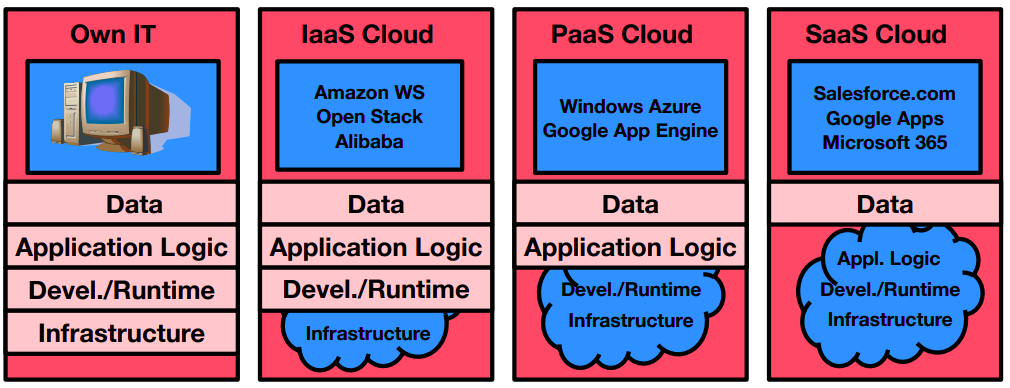
\includegraphics[width=\textwidth]{servicemodels.png}
	%\caption{Comparison over the service models}
\end{figure}
\begin{figure}[H]
	\centering
	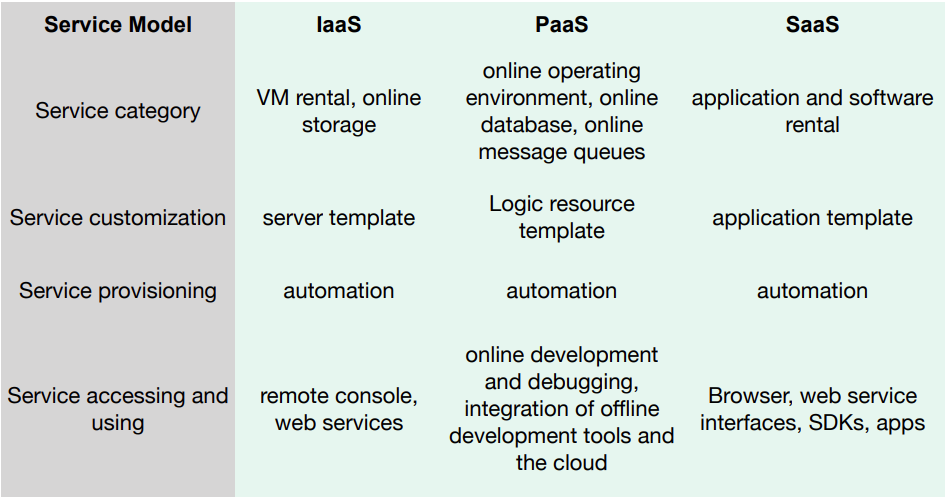
\includegraphics[width=0.8\textwidth]{servicemodel1.png}
	%\caption{Comparison over the service models}
\end{figure}\begin{figure}[H]
\centering
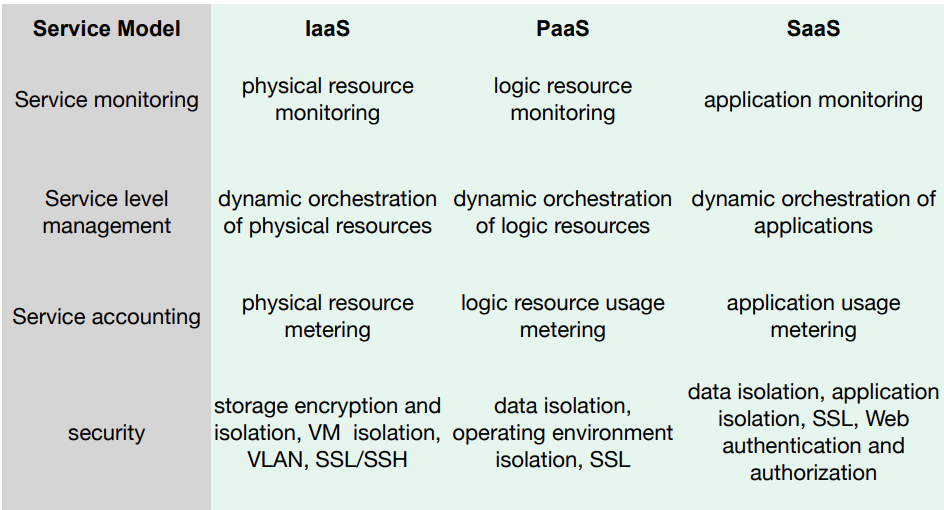
\includegraphics[width=0.8\textwidth]{servicemodel2.png}
%\caption{Comparison over the service models}
\end{figure}
\subsection{4 Deployment Models: Private, Community, Public, Hybrid}
\begin{itemize}
	\item Private Cloud:
	\begin{itemize}
		\item service offered \textbf{via private network} for \textbf{single client}.
	\end{itemize}
	\item Community Cloud:
	\begin{itemize}
		\item service offered to \textbf{a specific group of clients}.
	\end{itemize}
	\item Public Cloud:
	\begin{itemize}
		\item service offered \textbf{over Internet via Web-application} or third-party provider for \textbf{everyone}.
	\end{itemize}
	\item Hybrid Cloud: combination of public and private cloud.
\end{itemize}

\subsection{5 Essential Characteristics}
\begin{itemize}
	\item \textbf{on-demand self-service}: 
	\begin{itemize}
		\item able to \textbf{provision computing capabilities} unilaterally(no interaction required with provider).
	\end{itemize}
	
	\item \textbf{broad network access}: 
	\begin{itemize}
		\item capabilities can be available and accessed through by \textbf{diversely thin or thick client platforms} (mobile, tablets, cable, etc.)
	\end{itemize}
	
	\item \textbf{resource pooling}: 
	\begin{itemize}
		\item \textbf{multi-tenant model} is used, multiple customers shares the computing capabilities at the same time, according to their self-customized demand. Specification of resource location can be possible at higher abstraction level.
	\end{itemize}
	 
	\item \textbf{rapid elasticity}: 
	\begin{itemize}
		\item computing capabilities can be \textbf{elastically provisioned and released} in any quantity at any time. The process can be automated or scaled according to dynamic demand.
	\end{itemize}
	\item \textbf{measured service}: 
	\begin{itemize}
		\item automatically control and optimize resource use by \textbf{leveraging a metering capability}. Resource usage can be monitored, controlled and reported.
	\end{itemize}
\end{itemize}


\subsection{Pros \& Cons of Clouds}
\begin{itemize}
	\item Advantages:

\begin{itemize}
	\item scalability, elasticity
	\item rapid deployment
	\item no capital investment for physical resources
	\item outsourcing of infrastructure management
	\item limited access to on-premise servers
	\item fault tolerance: multiple servers have data replicas, if one node fails, other nodes will replace.
	\item collaboration
\end{itemize}
	\item Disadvantages:
	\begin{itemize}
		\item no control over security, based on ''trust''.
		\item no control over hardware/infrastructure
		\item vendor lockin: service is not standardized, not compatible to other vendors.
		\item cost on monthly fees: if demand for same computational power is constant, fee may be higher than building own hardware. Only recommendable for dynamic demand.
		\item breaking SLAs: your performance may be influenced by other tenants(multi-tenant model).
	\end{itemize}
\end{itemize}
	\section{Base Technologies of Clouds}
\subsection{Process Technology}
\paragraph{Production} the processors are produced from semi-conductor materials. It's primarily produced on a \textbf{waver} consisting of a lot of chips. Later the waver is cut after the production process. Individual chips will be packaged into the system.

\paragraph{Transistor} 
\begin{itemize}
	\item traditional 2D planar transistor: a 2D-planar structure, the gate controls how much current flows from source through the drain.
	\item 3D tri-gate transistor \textbf{FinFET}: conducting channels on 3 sides with a \textbf{vertical fin structure}. The width of a Fin is \textbf{10nm}, and it keeps shrinking.
\end{itemize}
The smaller the structure gets, the more transistors fit on the same space, the faster the transistor gets.

\subsection{Processor Architecture}

\subsubsection{CPU}
\begin{itemize}
	\item current state of CPU development:
	\begin{itemize}
		\item increase in transistors: up to 10nm or even 5nm.
		\item stop in increase of clock speed: up to 4GHz. Limitation: cooling. (the faster the clock speed, the more energy consumed, the hotter) 
		\item continuous need of performance improvement: parallelism on the chip, since halt in clock speed.
	\end{itemize}
	\item trends in CPU development:
	\begin{itemize}
		\item multi-core processors: parallelism
		\item SIMD support (Single Instruction, Multiple Data): parallelism inside of a single instruction, computation of vectors of values in parallel.
		\item combination of core private and shared caches:
		\begin{itemize}
			\item data saved in cache for repeated operations
			\item with multiple caches, cores can communicate. However, this may disturb the usage of cache.
			
		\end{itemize}
		\item hardware support for energy control: \textbf{dynamic voltage and frequency scaling}  
		\begin{itemize}
			\item chips work in a dynamic frequency controlled by hardware according to the need of the running software. 
			\item It checks whether operations are memory-bound or compute-bound.
		\end{itemize}
		   
		\item 64-bit architectures
		  
	\end{itemize}
	\item challenge: the \textbf{memory hierarchy}
	\begin{itemize}
		\item access to the main memory is slow, involving several hundreds of cycles for CPU, while each of these cycles can be responsible for multiple operations.
		
		$\rightarrow$ save such cycles for accessing data but keep the \textbf{data near to execution}.
		\item \textbf{Level-1 Instruction \& Data Cache}: fastest, but too slow to feed all data in large size. (64 Bytes: 8 double precision values, 64 bit long values)
		\item \textbf{Level-2 Unified Cache}: not separated, access better. 
		\item \textbf{Translation Lookaside Buffer (TLB)}: translates virtual addresses into physical addresses and loads into main memory, it only stores the \textbf{most recent translation}, no need to lookup constantly.
	\end{itemize}
	\begin{figure}[H]
		\centering
		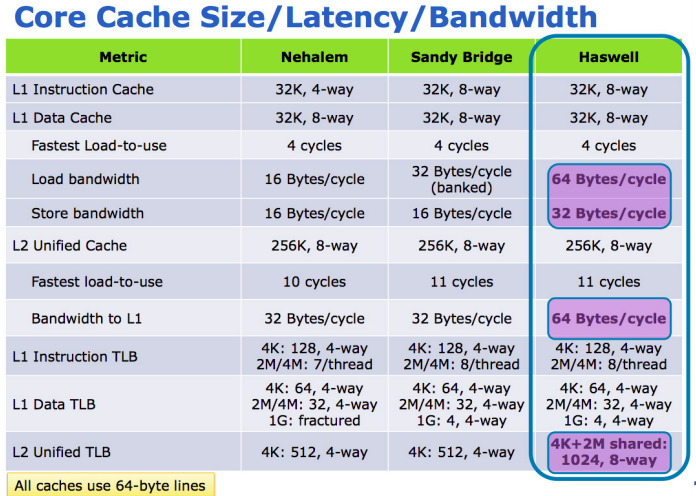
\includegraphics[width=0.65\textwidth]{memhier.png}
	\end{figure}
\end{itemize}

\subsubsection{Skylake Architecture} 

\begin{figure}[H]
	\centering
	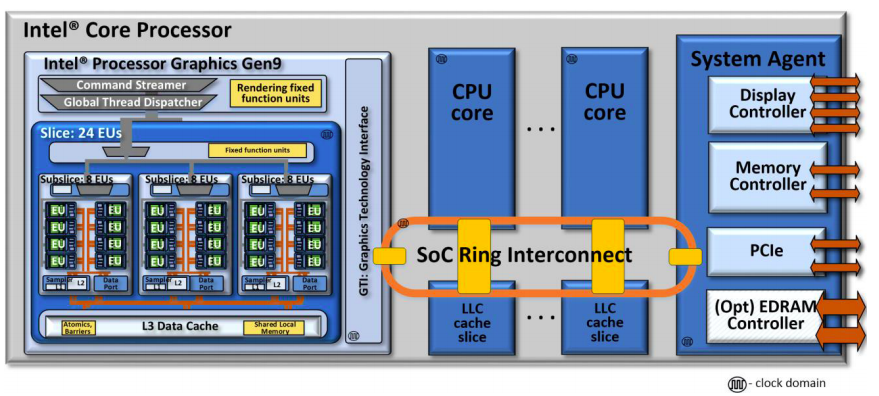
\includegraphics[width=0.7\textwidth]{skylake.png}
\end{figure}
The archiecture of a processor (one chip)
\begin{itemize}
	\item graphic processor: accelerator for specified computation
	\item system agent: support structures (eg: display controller, memory controller, PCIe for I/O, EDRAM controller)
	\item CPU cores: homogeneous cores with a \textbf{private cache each}.
	\item LLC cache slice: each slice cache is associated to each CPU core. 
	\begin{itemize}
		\item If core misses information in its private cache: through interconnect, it checks which slice cache contains the info, then it propagates to the cache associated the CPU core and returns the info back to the CPU.
	\end{itemize}
	
	\item SoC Ring interconnect: all parts are connected by a ring bust.
	\begin{itemize}
		\item if CPU writes to I/O device -- PCIe, it first puts information onto the bust, then it propagates into the PCIe and is written to the disk.
	\end{itemize}
\end{itemize}
$\rightarrow$ the \textbf{interconnect ring} is the \textbf{bottleneck} for increasing the cores.

$\rightarrow$ alternatives: Xeon Phi

\subsubsection{Xeon Phi Architecture} 
\begin{figure}[H]
	\centering
	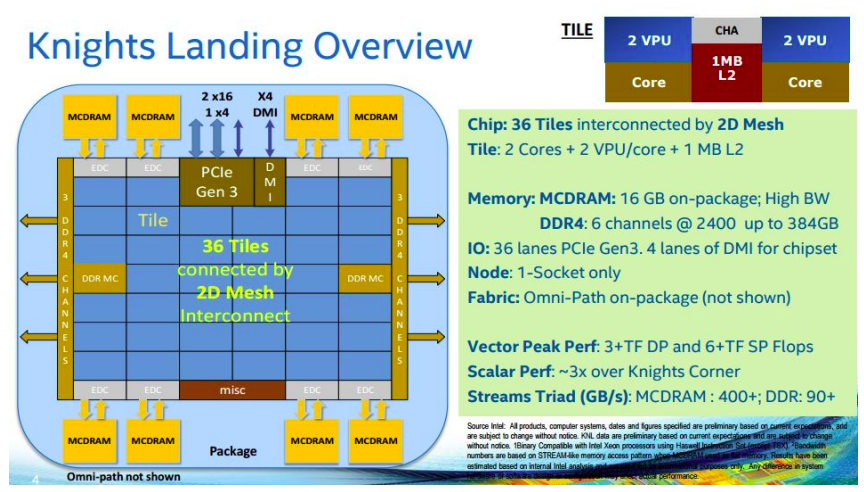
\includegraphics[width=0.7\textwidth]{xeonphi.png}
\end{figure}
\begin{itemize}
	\item Goal: allows significantly \textbf{more cores} in a single processor, in a single CPU die.
	\item Idea: 
	\begin{itemize}
		\item the die is organized into a \textbf{tile-architecture}.
		\item 36 compute tiles are connected through a \textbf{2D mesh network} $\rightarrow$ connection between tiles in both x- and y-direction.
		\item each tile has 2 cores $\rightarrow$ \textbf{72 cores} in total
	\end{itemize}
	\item Tile structure:
	\begin{itemize}
		\item 2 cores
		\item 2 VPUs (Vector Processing Unit) for each core $\rightarrow$ 4 in total per tile.
		\item L2 cache: shared between the cores, but as a private cache for each tile. 
		
		$\rightarrow$ multiple copies of an address can be in different private L2 caches of different tiles, which \textbf{must be coherent}.
		\item CHA (Caching Hold Agent): responsible for the \textbf{coherence}. It's connected to each tile, keeping track of the status of the copies by implementing a \textbf{coherence protocol}. 
	\end{itemize}
	\item Memory: 
	\begin{itemize}
		\item DDR4 memory
		\item \textbf{MCDRAM}-- Multi-channel DRAM, \textbf{high bandwidth}(450 GB/s)
		
		Memory modes:
		\begin{itemize}
			\item flat mode: all MCDRAM is used as \textbf{physical address}. Data structure can explicitly choose between MCDRAM or DDR. 
			\item cache mode: all MCDARM is used as \textbf{L3 cache}. physical addresses only on DDR. If data is being processed from DDR, it's mapped to MCDRAM.
			\item hybrid mode: combination of flat and cache mode. Part of MCDRAM is used as \textbf{L3 cache}, the other as \textbf{physical addresses}.
		\end{itemize}
		\begin{figure}[H]
			\centering
			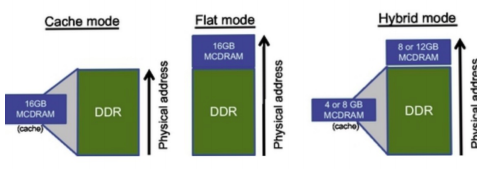
\includegraphics[width=0.65\textwidth]{memorymodes.png}
		\end{figure}
	\end{itemize}	
\end{itemize}

\subsubsection{Processors for mobile devices: ARM}
\begin{figure}[H]
	\centering
	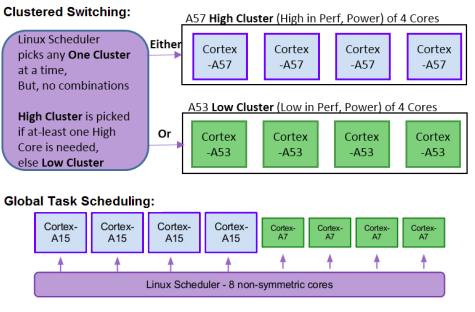
\includegraphics[width=0.65\textwidth]{arm.png}
\end{figure}
\begin{itemize}
	\item \textbf{Big Little Principle}
	\begin{itemize}
		\item Combination of \textbf{high clusters} and \textbf{low clusters}, controlled by clustered switching. 
		\begin{itemize}
			\item high cluster: high in performance
			\item low cluster: low in performance, but energy efficient
			\item only \textbf{one cluster} at a time, \textbf{no combinations}.
		\end{itemize}
		\item Global task scheduling: tasks are scheduled according to the requirement between 2 clusters.
	\end{itemize}
	\item Use-cases: Apple Processor A14 (2 high performance Firestorm, 2 energy-efficient Icestorm)
\end{itemize}


\subsection{Accelerator Programming}
\begin{itemize}
	\item Motivation: 
	\begin{itemize}
		\item increase computational speed and reduce energy consumption
		
		$\rightarrow$ achieved by \textbf{specialization} in operations/on-chip communication/memory accesses
		
		$\rightarrow$ \textbf{accelerator}
	\end{itemize}
	\item Types:
	\begin{itemize}
		\item GPGPU (General Purpose Graphic Processors)
		\item FPGA
		\item standard cores
	\end{itemize}
	\item Designs:
	\begin{itemize}
		\item CPU with accelerators attached: computation can be offloaded onto the accelerator.
		\item accelerators-only design
		\item accelerator booster: a collection of accelerators as a separate part from the whole system. Jobs can be computed by these accelerators when necessary. Accelerator booster can be shared among parallel jobs.
	\end{itemize}
	
\end{itemize}

\subsubsection{Graphic Processing Units (GPU)}
\begin{itemize}
	\item Usage: 
	\begin{itemize}
		\item visualization
		\item \textbf{general processing} (NVIDIA)
	\end{itemize}
	\item Parallelism: multi-threading, MIMD, SIMD
	\item Challenges:
	\begin{itemize}
		\item a \textbf{specialized programming interface} for the GPGPU needed (eg: CUDA from NVIDIA)
		\item \textbf{scheduling coordination} on system processor and GPU
		\item \textbf{transfer of data} between system memory and GPU memory
	\end{itemize} 
	\item example: NVIDIA Tesla P100
\end{itemize}

\paragraph{NVIDIA Tesla P100}
\begin{itemize}
	\item GP100 (GPU):
	\begin{itemize}
		\item L2 cache: shared among all compute units --  streaming multi-processor
		\item NVLink: able to connect multiple GPGPUs together
		\item memory controller: access to high bandwidth memory
		\item 6 Graphic Processing Clusters(GPC)
			\begin{itemize}
				\item 10 Streaming Multi-Processor each GPC, 60 in total
				\item 5 Textural Processing Clusters (TPC), 1 for 2 SM, 30 in total
			\end{itemize}
		\end{itemize}

		\item High Bandwidth Memory (HBM)
		\begin{itemize}
			\item \textbf{vertical stacks} of memory dies connected by microscopic wires
		
			$\rightarrow$ near and tight connection between memories
			\item 180 GB/s per stack bandwidth
		\end{itemize}
\end{itemize}

$\rightarrow$ good for data parallel processing like vector processing.

\subsubsection{Field Programmable Gate Arrays (FPGA)}
\begin{itemize}
	\item hardware which is programmable
	\item Consist of:
	\begin{itemize}
		\item \textbf{array of logic gates} to implement \textbf{hardware-programmed special functions}
		\item \textbf{specialized functional units} (eg: signal processors, multipliers)
		\item static \textbf{memory}
	\end{itemize}
	\item programmed in VHDL: the program describe functions to be executed, it will then be translated into look-up tables, which are put into the logic gates
	\item Use-case:
	\begin{itemize}
		\item as \textbf{accelerator} for specialized computations
		\item \textbf{filtering} for databases
		\item as \textbf{switches, routers} for communication
		\item \textbf{preprocessing}: I/O hardware of FPGA accesses the DDR, local computation can be organized in the pipeline of FPGA. Local preprocessing will be done on FPGA and the output will be sent ot external processor via PCIe.
	\end{itemize}
	\item examples: Altera, Xilinx
\end{itemize}

\subsection{Architecture for Parallelism: Shared Memory Systems}
\begin{itemize}
	\item Idea: 2 architectures to \textbf{achieve parallelism}, which is combining multiple processors together for computation. 
	\begin{itemize}
		\item shared memory system
		\item distributed memory system
	\end{itemize}
	\item \textbf{Non-Uniform Memory Access (NUMA)}:
	\begin{itemize}
		\item \textbf{multiple CPU} with multiple cores are connected through \textbf{single physical address} space.
		
		$\rightarrow$ access time depends on the \textbf{distance to the physical address} (memory)
		
		$\rightarrow$ CPU accesses either local(near) or remote memory $\rightarrow$ locate the memory near for fast access.
	\end{itemize}
	\paragraph{Example: SuperMUC}
	
	\begin{itemize}
		\item 2 multi-core processors(Sandy Bridge) with 32GB memory in total
		\item each processor can access to all 32GB memory, \textbf{however access time differs}
		\item \textbf{Latency}
		\begin{itemize}
			\item local: $\sim$50ns, $\sim$135 cycles
			\item remote: $\sim$90ns, $\sim$240 cycles
		\end{itemize}
		
	\end{itemize}
	\begin{figure}[H]
		\centering
		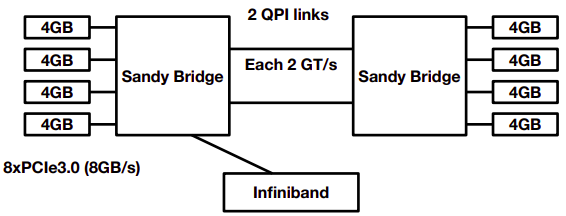
\includegraphics[width=0.65\textwidth]{numa.png}
	\end{figure}

	\item Programming interfaces for Shared Memory Systems
	\begin{itemize}
		\item explicit threading
		\item automatic parallelization: sequential code is given to compiler, which \textbf{automatically} parallelize the work among available CPUs.
		\item OpenMP: directive-based parallel programming, parallel computations are \textbf{explicitly expressed}.
	\end{itemize}
	\item Challenges in parallel computing:
	\begin{itemize}
		\item explicit synchronization needed.
		\item \textbf{cocurrency bugs}: the outcome of the computation depends on the speed of access to the memory $\rightarrow$ non-deterministic results possible.
		\item control of \textbf{data locality}
	\end{itemize}
\end{itemize}

\subsection{Architecture for Parallelism: Distributed Memory Systems}
\begin{itemize}
	\item Characteristics
	\begin{itemize}
		\item \textbf{Coupling} of individual nodes via network: processor only have access to the memory in node.
		\item \textbf{no shared} physical address space
		\item communication between nodes: transfer of \textbf{messages}
	\end{itemize}
	\item Programming in Distributed Memory Systems: \textbf{more difficult} than shared memory systems.
	\begin{itemize}
		\item + : \textbf{rare race conditions} $\rightarrow$ cocurrency bugs low.
		\item -- : Message Passing Interface(MPI), have to explicitly decompose or insert message passing $\rightarrow$ more difficult to program.
		\item Process to Process communication and collective operations
	\end{itemize}
	\item Challenges: 
	\begin{itemize}
		\item \textbf{more difficult} to programm than shared memory systems
		\item \textbf{expensive communication}, much slower than access to memory.
		$$t(message) = \text{startup time} + \frac{\text{message size}}{\text{bandwidth}}$$
		\begin{itemize}
			\item communication with one large message is more efficient than multiple small messages (startup time)
			\item mapping onto processors has performance impact. Communication may not need to go through the entire but locally. (eg: 2D mesh network)
		\end{itemize}
	\end{itemize}
\end{itemize}

\subsection{Data Center Networks}
Inside the data center, the \textbf{servers} are connected by \textbf{LAN}-- Local Area Network. Each \textbf{server} is connected to a \textbf{switch}. The \textbf{switches} are connected, which allows \textbf{communication between the servers}. \\ \ \\

Multiple \textbf{LANs} are possible in a data center. The \textbf{LANs} can be connected through a \textbf{router}. A router is based on a IP-address, it can make decisions depending on the IP-address (eg: receiver of message). \\ \ \\

The \textbf{routers} in the data center can be connected to a \textbf{WAN}-- Wide Area Network, the internet. The \textbf{WAN} can be connected to a \textbf{local router}, which a client has access to . This is the \textbf{last mile} to reach the client, frequently \textbf{radio network} is used -- WLAN or GSM.

\subsubsection{Different Networks}
\begin{itemize}
	\item Types:
	\begin{itemize}
		\item WAN -- Wide Area Networks
		\begin{itemize}
			\item homogeneous base technology (opto-electronic)
		\end{itemize}
		
		\item LAN -- Local Area Networks and Cluster Networks
		\begin{itemize}
			\item non-shared Ethernet
			\item Infiniband
		\end{itemize}
		
		\item Last Mile
		\begin{itemize}
			\item heterogeneous base technology (Radio, TV cables, etc.)
		\end{itemize}
	\end{itemize}

	\item Performance Metrics:
	\begin{itemize}
		\item \textbf{Latency}: transport time of a message
		\begin{itemize}
			\item physical delay: time needed to go through the links, limited by speed of light, \textbf{not optimizable}.
			\item protocol delay: time needed to execute protocol operations. \textbf{compensated by increase of CPU performance.}
			\item line waiting time: time to wait until the link is available. negligible up to 10\% utilization. \textbf{reduced by increasing bandwidth}.
			\item transmission time: time needed to send certain amount of data over the link. \textbf{reduced by increasing bandwidth}.
			$$\text{transmission time} = \frac{\text{message size}}{bandwidth}$$
		\end{itemize}
		\item \textbf{Bandwidth} (byte/sec): the speed transporting a message
	\end{itemize}
\end{itemize}


\subsubsection{Local Area Network}
\paragraph{Ethernet}
\begin{itemize}
	\item first implementation based on a \textbf{shared cable}: all computer are connected through one cable. Only one computer can transmit message at a time.
	\item now \textbf{switched Ethernet}: each computer is connected to a switch. Switches are connected together to enable communication. A switch replicates all packets to all ports.
	\item Speed: 10 Mbit/s, 100 Mbit/s or 1000 Mbit/s
\end{itemize}

\paragraph{VLAN -- Virtual Local Area Network}
\begin{itemize}
	\item Characteristics:
	\begin{itemize}
		\item a single LAN is \textbf{partitioned} into \textbf{multiple virtual LANs}.
		
		$\rightarrow$ direct traffic or for security reasons.
		\item each virtual LAN is a \textbf{single broadcast domain}
		\item \textbf{communication} between VLANs only through \textbf{router} 
	\end{itemize}

	\item \textbf{Port-based VLAN}
	\begin{itemize}
		\item The \textbf{ports} of a switch are \textbf{specifically assigned} to a \textbf{VLAN}.
		\item servers of a VLAN from two switches are communicated through a \textbf{link}.
		\item  \# links = \# VLANs
	\end{itemize}
	
	\item \textbf{Tagged VLAN}
	\begin{itemize}
		\item one port of a switch is not connected to server. This port is connected to other switches through a \textbf{link}. This link manages all packets.
		\item \textbf{Tag}: packets are \textbf{only forwarded to ports with the same tag}.
		\item \# links = 1
	\end{itemize}
\end{itemize}

\paragraph{Infiniband}
\begin{itemize}
	\item Characteristics:
	\begin{itemize}
		\item low latency, high bandwidth
		\item speed: 25 Gbit/s
		\item RDMA access: \textbf{direct access of memory of other computer}. Instead of packing data into a message an sending to the operation system and then taking it out, RDMA can \textbf{directly fetch} the data from memory and forward it to the requester. 
		
		No protocol overhead or handling of message $\rightarrow$ \textbf{faster}.
		\item based on \textbf{Virtual Interface Adapter}: data transfer don't require operation system support.
	\end{itemize}
	\item Use-case: clusters and servers
\end{itemize}

\subsubsection{Software-defined Networks}
\begin{itemize}
	\item Motivation:
	\begin{itemize}
		\item higher speed
		\item automated network configurations
		\item security
		\item adaptation to performance variations
	\end{itemize}
	\item Current network management:
	\begin{itemize}
		\item Management plane --> Control plane --> Data/Forwarding plane
	\end{itemize}
	\item Software Defined Networking:
	\begin{itemize}
		\item allows network administrators to \textbf{programmatically initialize, control, change and manage the network behavior dynamically} via open interfaces
		\item Protocol: OpenFlow
		\begin{itemize}
			\item enables an open interface to \textbf{interact} with networking devices (machines, switches from different providers)
			\item network layers on top of L3
			\item SDN controllers communicate to L3 switches using openFlow protocols. 
		\end{itemize}
	\end{itemize}

\end{itemize}


\subsubsection{Last Mile Networks}

\paragraph{Wireless Local Area Network -- WLAN}
\begin{itemize}
	\item consists of \textbf{clients} and \textbf{access points} as routers.
	\item modes:
	\begin{itemize}
		\item \textbf{infrastructure}: clients connect to the access point
		\item \textbf{ad hoc}: clients communicate with each other
	\end{itemize}
	\item Security:
	\begin{itemize}
		\item Wireless Equivalent Privacy (WEP)
		\item Wi-Fi Protected Access (WPA1, WPA2) 
	\end{itemize}
	\item Speed:
	\begin{itemize}
		\item 802.11 n: 800 Mbit/s, 70m
		\item 802.11 ac: 1733 Mbit/s, 35m
	\end{itemize}
\end{itemize}

\paragraph{Digital Subscriber Line -- DSL}
\begin{itemize}
	\item transmission of data \textbf{over telephone lines}, share with telephone service (different frequency)
	\item Speed:
	\begin{itemize}
		\item asymmetric DSL: upstream bandwidth \textbf{much lower} than downstream
		\item downstream: 256 Kbit/s to 100 Mbit/s
	\end{itemize}
	
\end{itemize}

\paragraph{Very-high-bit-rate Digital Subscriber Line -- VDSL}
\begin{itemize}
	\item higher speed than DSL:
	\begin{itemize}
		\item different versions: VDSL, VDSL2, VDSL2-Vplus
		\item VDSL: up to 55Mbit/s downstream, 16 Mbit/s upstream 
	\end{itemize}
	\item VDSL with \textbf{vectoring}: reduce crosstalk between different lines. (Crosstalk: communication on one line influences the communciation on other lines)
	
	$\rightarrow$ special encoding of neighbouring lines: a provider needs to have \textbf{access to all lines in a bundle}
	
	$\rightarrow$ current implementation difficult
\end{itemize}

\paragraph{Global System for Mobile Communication --GSM}
\begin{itemize}
	\item network for \textbf{mobile phones}, 3G, 4G, 5G
	\item access to the network using SIM card
\end{itemize}

\subsection{Storage Technologies}
\begin{figure}[H]
	\centering
	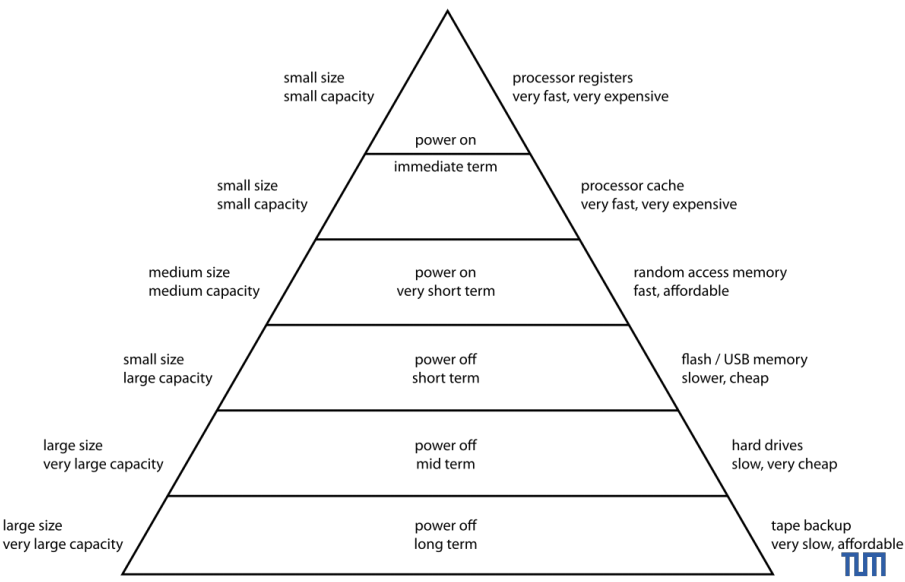
\includegraphics[width=0.8\textwidth]{storage.png}
\end{figure}
\subsubsection{Local Storage}

\paragraph{Redundant Array of Independent Disks -- RAID}
\begin{itemize}
	\item Goal: increase reliability or bandwidth
	\item RAID 0: \textbf{distribute} blocks over \textbf{2 disks}, if \textbf{write both blocks on two disks} at the same time, it gets \textbf{double bandwidth} to the disk.
	
	$\rightarrow$ \textbf{higher bandwidth}
	\item RAID 1: \textbf{replicates} blocks on \textbf{2 disks}. If one fails, we still have the information on the other disk. 
	
	$\rightarrow$ \textbf{higher reliability}
	\item RAID 5: \textbf{distribute} blocks over \textbf{4 disks}, while one disk saves the \textbf{parity information}. If one block fails, the parity information enables \textbf{reconstruction}. Parity information of blocks is not written on the same disk, but \textbf{distributed} over all disks.
	
	$\rightarrow$ \textbf{higher bandwidth and reliability}
\end{itemize}
\paragraph{Flash}
\begin{itemize}
	\item non-volatile memory, retains stored information even after power is removed.
	\item Write operation: tunnel injection, a high positive voltage between control gate and source \textbf{pushes electrons into the floating gate}. It stays/saves in the floating gate as stored information. 
	\item Read operation: a higher voltage is required at the drain to make the channel conduct, the electrons move from source to drain.
	\item Increasing storage density: \textbf{increase floating gates} in a flash cell
	\begin{itemize}
		\item Single Level Cells (SLC): stores \textbf{1 bit} of information
		\item Multiple Level Cells (MLC): stores \textbf{2 bits} of information
		\item \# floating gates $\uparrow$, cost per bit $\downarrow$, storage density $\uparrow$, program-erase cycles $\downarrow$, write/reading speed $\downarrow$
	\end{itemize}
	
	\item Use-case: USB-disks, SD-cards, mobile phone storage, built in SSD
\end{itemize}

\paragraph{SSD}
\begin{itemize}
	\item Comparison with hard disks:
	\begin{itemize}
		\item lower latency, random access
		\item smaller storage capacity
		\item less power hungry
		\item faster read/write speed
	\end{itemize}
\end{itemize}

\subsubsection{Data Center Storage}
\begin{itemize}
	\item storage comparison: \euro/IOPS 
	\item only based on flash storage or SSDs, combined with RAID, with special controllers optimized for SSDs.
	
	$\rightarrow$ IOPS $\uparrow$, latency $\downarrow$, bandwidth $\uparrow$, cost $\uparrow$
\end{itemize}


\subsubsection{Provisioning of Storage}
\begin{itemize}
	\item 3 ways to provide storage:
	\begin{itemize}
		\item Direct Attached Storage: storage devices are attached to the individual computer
		\item Storage Area Network
		\item Network Attached Storage
	\end{itemize}
\end{itemize}


\paragraph{Storage Area Network -- SAN}
\begin{itemize}
	\item access to \textbf{block level} data storage
	\item a \textbf{specialized network} connecting the servers which separates from LAN
	\item \textbf{no pre-existing file system}, the server can define its own file system according to needs
	\item a shared pool of spare resources, which allows \textbf{flexible allocation of spare storage} 
	
	\item Advantages:
	\begin{itemize}
		\item \textbf{flexible distribution} of devices between clients, reconfiguration of distribution in software instead of adaptation of cabling.
		\item easy replacement of faulty servers
		\item back-up can be done centrally, easier disaster protection
		\item no pre-existing file system, allows \textbf{customization} according to needs.
	\end{itemize}
	Disadvantages:
	\begin{itemize}
		\item shared network bandwidth
		\item shared performance of storage devices
	\end{itemize}
\end{itemize}
\begin{figure}[H]
	\centering
	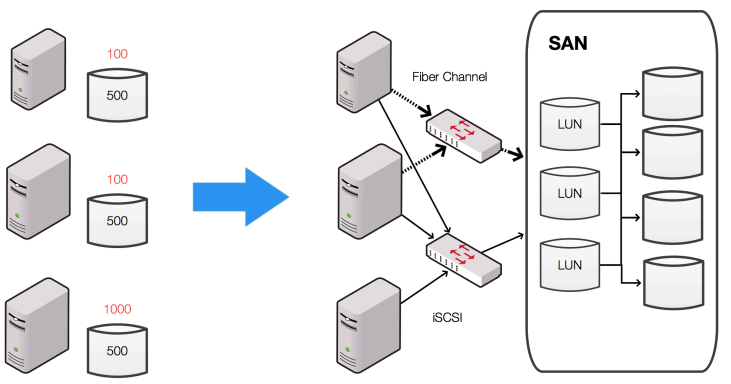
\includegraphics[width=0.7\textwidth]{san.png}
\end{figure}

\paragraph{Network Attached Storage -- NAS}
\begin{itemize}
	\item storage devices(disks) are connected to a \textbf{file server}
	\item computers \textbf{go over the network} and \textbf{access the file system} on file server
	\item an \textbf{existing file system}.
	\item network file sharing protocols: NFS
	\item storage devices: RAID to increase bandwidth and reliability
	\item Use-case: streaming contents(movies, images) to home network. If connected to home WiFi, then access to local storage. Access out of home using VPN and public IP
	
\end{itemize}
\begin{figure}[H]
	\centering
	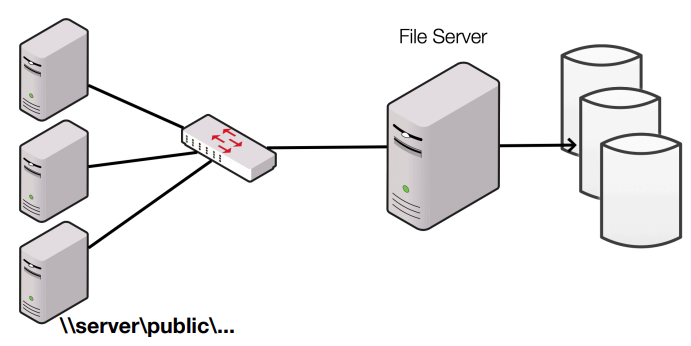
\includegraphics[width=0.7\textwidth]{nas.png}
\end{figure}


\subsubsection{Storage Virtualization}
\begin{itemize}
	\item Goal: location transparency
	\item Process: allocate a \textbf{virtual disk}, which will be \textbf{mapped to a real physical hard-disk} in the Storage Area Network. The \textbf{client won't know about which hard-disk is allocated} for the virtual disk.
\end{itemize}
\paragraph{Block Virtualization}
\begin{itemize}
	\item the \textbf{mapping} of a \textbf{virtual disk and block number} to a \textbf{physical disk and block number}.
	\item Use-case: SAN, flexible mapping, disk expansion and shrinking
	\item implementation:
	\begin{itemize}
		\item host based: host runs virtualization software
		\item storage device based: disk array provides a virtualization level
		\item \textbf{network based}: virtualization device is in LAN and connected to a SAN, \textbf{most frequent implementation}
		\begin{itemize}
			\item \textbf{in-band}: client sends request for certain blocks to the controller in the network, the controller fetches the data and returns the data to the client.
			\item \textbf{out-of-band}: host contacts the controller, gets the mapping information and accesses the data in SAN directly without the help of controller.
		\end{itemize}
	\end{itemize}
\end{itemize}

\paragraph{File Virtualization}
\begin{itemize}
	\item Virtualization on \textbf{file level}
	\item Use-case: \textbf{Distributed File System}
	\begin{itemize}
		\item allows transparent access to multiple NAS server. Files located on multiple NAS servers \textbf{appears as if on a single NAS}, the client doesn't know on which server the file exists.
	\end{itemize} 
\end{itemize}

\end{document}
